\documentclass{article}
\usepackage[utf8]{inputenc}
\usepackage{fancyhdr}
\usepackage{lastpage}
\usepackage{amsfonts}
\usepackage{amsmath}
\usepackage{amssymb}
\usepackage{bm}
\usepackage{bbm}
\usepackage{tikz}

\usetikzlibrary{shapes}
\usetikzlibrary{automata, positioning, arrows}

\usepackage[shortlabels]{enumitem}
\usepackage[noabbrev, capitalise]{cleveref}

\usepackage{geometry}
 \geometry{
 a4paper,
 top=20mm,
 bottom=25mm,
 left=25mm,
 right=25mm,
 }

% define your IDs here:
\newcommand{\firststudentid}{341438711}
\newcommand{\secondstudentid}{321082026}

\pagestyle{fancy}
\fancyhf{}
\rhead{Written Solution for Assignment 4}
\chead{\firststudentid \qquad \secondstudentid}
\lhead{Natural Language Processing}
\rfoot{Page \thepage \hspace{1pt} of \pageref{LastPage}}
\renewcommand{\footrulewidth}{1pt}
 
\setlength{\parindent}{0pt}
\setlength{\parskip}{1em}
\renewcommand{\baselinestretch}{1.25}

\renewcommand{\thesubsection}{\thesection.\alph{subsection}}
\renewcommand{\thesubsubsection}{\thesubsection.\roman{subsubsection}}

\begin{document}

\section*{1. Neural Transition-Based Dependency Parsing}
\paragraph{b}
A parsing process of a sentence "I parsed this sentence
correctly":

\begin{table}[h!]
\begin{tabular}{|l|l|l|l|l}
\cline{1-4}
\textbf{Stack}                    & \textbf{Buffer}                            & \textbf{New dependency} & \textbf{Transition}   &  \\ \cline{1-4}
{[}ROOT{]}                        & {[}I, parsed, this, sentence, correctly{]} &                         & Initial Configuration &  \\ \cline{1-4}
{[}ROOT, I{]}                     & {[}parsed, this, sentence, correctly{]}    &                         & SHIFT                 &  \\ \cline{1-4}
{[}ROOT, I, parsed{]}             & {[}this, sentence, correctly{]}            &                         & SHIFT                 &  \\ \cline{1-4}
{[}ROOT, parsed{]}                & {[}this, sentence, correctly{]}            & parsed $\rightarrow$ I                & LEFT-ARC              &  \\ \cline{1-4}
{[}ROOT, parsed, this{]}          & {[}sentence, correctly{]}                  &                         & SHIFT                 &  \\ \cline{1-4}
{[}ROOT, parsed, this,sentence{]} & {[}correctly{]}                            &                         & SHIFT                 &  \\ \cline{1-4}
{[}ROOT, parsed, sentence{]}      & {[}correctly{]}                            & sentence $\rightarrow$ this           & LEFT-ARC              &  \\ \cline{1-4}
{[}ROOT, parsed{]}                & {[}correctly{]}                            & parsed $\rightarrow$ sentence         & RIGHT-ARC             &  \\ \cline{1-4}
{[}ROOT, parsed,correctly{]}      & {[}{]}                                     &                         & SHIFT                 &  \\ \cline{1-4}
{[}ROOT, parsed{]}                & {[}{]}                                     & parsed $\rightarrow$ correctly        & RIGHT-ARC             &  \\ \cline{1-4}
{[}ROOT{]}                        & {[}{]}                                     & ROOT $\rightarrow$ parsed             & RIGHT-ARC             &  \\ \cline{1-4}
\end{tabular}
\end{table}

\paragraph{c}
Each word must be added to stack, i.e. it's n SHIFT steps. \\
Each word must be dependent on other word, i.e. it's n RIGHT/LEFT-ARC steps. \\
One step for connecting to the ROOT. In total 2n+1 steps. \\

\paragraph{g} Training results: \\
dev UAS: 88.45 \\
test UAS: 88.83 \\

\paragraph{h}
\begin{enumerate}
\item
"It is on loan from a guy named Joe O’Neill in Midland , Texas" \\
    Error Type: Prepositional Phrase Attachment Error \\
    Incorrect dependency: named $\rightarrow$ Midland \\
    Correct dependency: guy $\rightarrow$ Midland \\

\item
"Brian has been one of the most crucial elements to the success of Mozilla software ." \\
    Error Type: Modifier Attachment Error \\
    Incorrect dependency: elements $\rightarrow$ most \\
    Correct dependency: crucial $\rightarrow$ most \\

\item
"I was heading to a wedding fearing my death" \\
    Error Type: Verb Phrase Attachment Error \\
    Incorrect dependency: wedding $\rightarrow$ fearing \\
    Correct dependency: heading $\rightarrow$ fearing \\
    
\item
"It makes me want to rush out and rescue people from dilemmas of their own making." \\
    Error Type: Coordination Attachment Error \\
    Incorrect dependency: makes $\rightarrow$ rescue \\
    Correct dependency: rush $\rightarrow$ rescue \\
\end{enumerate}

\section*{2. Syntactic Parsing}

\begin{itemize}
    \item[(a)] The long sentences are caused by the rules $NP \to NP \  PP$ and $PP \to Prep \ NP$, as these rules can apply recursively an infinite number of times. 

    In particular, the first rule $NP \to NP \  PP$  contains the nonterminal symbol $NP$ on both the left and right hand sides, so it may be applied an infinite number of times.

    The second rule can also be used to create infinite recursion by expanding $NP$ to $NP \  PP$ (rule 1) to $NP \ Prep \ NP$ (rule 2),

    \item[(b)] At each iteration of the generation algorithm, a nonterminal is expanded by choosing a random expansion in proportion to their weights. The preterminal symbol $Noun$ has six expansions in the grammar, each of weight one ($Noun \to Adj \ Noun$, $Noun \to president$, $Noun \to airline$, etc.). Therefore every noun has only probability $1/6$ of being preceded by at least one adjective, probability $1/36$ of being preceded by at least two adjectives, and so forth (geometric distribution).

    \item[(c)] The problem in (a) could be fixed by reducing the weight of the rule $NP \to NP \  PP$ (or increasing the weights of all other rules expanding $NP$). The problem in (b) could be fixed by increasing the weight of the rele $Noun \to Adj \ Noun$ (or decreasing the weight of all other rules expanding preterminal $Noun$).

    \item[(d)] (implemented in cky.py)

    \item[(e)] Output parse: (S (NP (Det the) (Noun president)) (VP (Verb ate) (NP (Det the) (Noun (Adj delicious) (Noun sandwich)))))

\end{itemize}

\section*{3. Semantic Parsing}

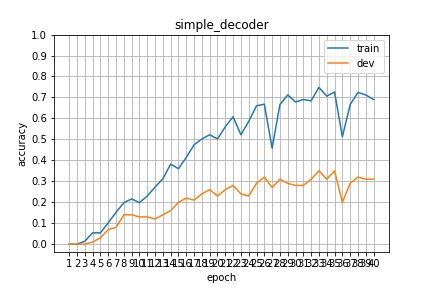
\includegraphics[scale=0.5]{simple_decoder.png}

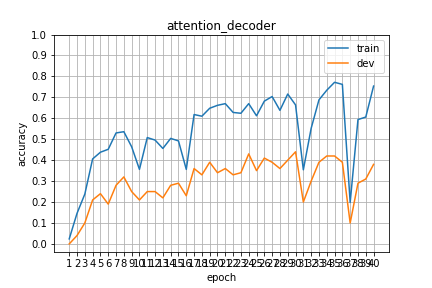
\includegraphics[scale=0.5]{attention_decoder.png}

\end{document}